%%%%%%%%%%%%%%%%%%%%%%
\documentclass{singlecol-new}
%%%%%%%%%%%%%%%%%%%%%%

\usepackage{natbib,stfloats}
\usepackage{mathrsfs}
\def\newblock{\hskip .11em plus .33em minus .07em}
\theoremstyle{TH}{
\newtheorem{lemma}{Lemma}
\newtheorem{theorem}[lemma]{Theorem}
\newtheorem{corrolary}[lemma]{Corrolary}
\newtheorem{conjecture}[lemma]{Conjecture}
\newtheorem{proposition}[lemma]{Proposition}
\newtheorem{claim}[lemma]{Claim}
\newtheorem{stheorem}[lemma]{Wrong Theorem}
\newtheorem{algorithm}{Algorithm}
}

\theoremstyle{THrm}{
\newtheorem{definition}{Definition}[section]
\newtheorem{question}{Question}[section]
\newtheorem{remark}{Remark}
\newtheorem{scheme}{Scheme}
}

\theoremstyle{THhit}{
\newtheorem{case}{Case}[section]
}

\makeatletter
\def\theequation{\arabic{equation}}





  %  International Journal of Computational Vision and Robotics


%\JOURNALNAME{\TEN{\it Int. J. Computational Vision and Robotics

%Vol. \theVOL, No. \theISSUE, \thePUBYEAR\hfill\thepage}}%
%
%\def\BottomCatch{%
%\vskip -10pt
%\thispagestyle{empty}%
%\begin{table}[b]%
%\NINE\begin{tabular*}{\textwidth}{@{\extracolsep{\fill}}lcr@{}}%
%\\[-12pt]
%Copyright \copyright\ 2012 Inderscience Enterprises Ltd. & &%
%\end{tabular*}%
%\vskip -30pt%
%%%\vskip -35pt%
%\end{table}%
%}
\makeatother








%%%%%%%%%%%%%%%%%
\begin{document}%
%%%%%%%%%%%%%%%%%

\setcounter{page}{1}

%\LRH{S.Chitra  et~al.}

\RRH{Computing disparity map using Minimum Sum Belief Propagation for stereo pair images}

\VOL{x}

\ISSUE{x}

\PUBYEAR{201X}

\BottomCatch

\CLline
\subtitle{}

\title{Computing disparity map using Minimum Sum Belief Propagation for stereo pair images}








%
%\authorA{Chitra Suresh}
%%
%\affA{Department of Electronics Engineering,\\RamRao Adik Institute of Technology,\\ Navi Mumbai ,India\\
%Fax: +1 \qquad E-mail:chitra.suresh@rait.ac.in}
%%NaviMumbai,India
%%
%\authorB{Kushal R. Tuckley}
%\affB{Department of Electrical Engineering,\\ Indian Institute of Technology ,\\ Powai ,India \\
%Fax: +1 \qquad E-mail:kushal@ee.iitb.ac.in  }
%%
%
%
%
%
%
%


%
%\authorA{Fusheng Wang\footnote{Work done while working at Siemens Corporate Research.} }
%
%\affA{Department of Biomedical Informatics, Emory University
%\newline
%36 Eagle Row, Ste 589, Atlanta, GA 30322, USA}
%
%
%
%\authorB{\footnotesize Cristobal Vergara-Niedermayr\footnote{Work done while working at Siemens Corporate Research.}}
%\affB{Oracle \newline
 %New Jersey, USA}
%
%
%\authorC{Peiya Liu}
%\affC{Department of Integrated Data Systems, Siemens Corporate
%Research \newline 755 College Road East, Princeton 08540, USA}








\begin{abstract}
Stereo matching between two images is done by computing disparity of all  points on the object. The process involves identifying corresponding points and finding the shift. Presently  there is no method that finds the shift in the corresponding point or points showing corresponding objects. This is mainly due  to non availability of                         procedure to identify the group of pixel from the same object. The local method either uses window or feature to find shift in a stereo image and  the  issues in local method are size of   window or extraction of feature. The global method uses graph theory and probability theory to find the shift efficiently. The belief propagation algorithm is one of the global methods expected to offer computationally efficient approach with good results. This paper has applied "Minimum Sum Belief Propagation" method for message updates with linear "Quadratic function ". The results with the computational estimations are presented below.
\end{abstract}








\KEYWORD{   stereo image; Stereo matching ; Belief propagation }








%\REF{to this paper should be made as follows: Rodr\'{\i}guez
%Bol\'{\i}var, M.P. and Sen\'{e}s Garc\'{\i}a, B. (201X) `The
%corporate environmental disclosures on the internet: the case of
%IBEX 35 Spanish companies', {\it International Journal of Metadata,
%Semantics and Ontologies}, Vol. x, No. x, pp.xxx\textendash xxx.}








%\begin{bio}Chitra Suresh received  A.M.I.E. degree in Electronics and communication engineering from the Institution of Engineers (India), Calcutta, India, in 1998, and  M.E. (electronics) from university of Mumbai, Mumbai, India in 2011. Her current research interests include Signals and Systems, Communication, Inference Algorithm ,High frequency circuits, Microelectronics and Image Processing. She is a Life Member of the Indian Society for Technical Education (ISTE)
%\vs{9}
%
%
%
%
%
%
%
%
%\noindent Kushal R. Tuckley received the B.Tech, M.Tech and Ph.D. degrees from the Indian Institute of Technology (IIT) Bombay, Mumbai, India, in 1985, in 1988 and 2009, respectively. His research interests are Radars, Microwave Systems, Image Processing and Wireless Industrial Instrumentation.\vs{8}
%
%
%
%
%
%
%
%
%\noindent
%\end{bio}
















\maketitle
















 \section{Introduction}








%The needs for data sharing
The parallax effect (ability to see an object at two different views) is present in stereoscopic or stereo pair image. The objects near the camera will represent more to the right in the left image and more to the left in the right image due to the parallax effect in stereoscopic or stereo pair   image. To find the horizontal matching pixel in the left and right image for stereo pair image is known as \textbf{stereo vision, stereo correspondence or stereo matching}. The horizontal pixel distance for each pixel coordinates is the disparity map or the depth map.\\
In practice, where occluded objects are in stereo pair image, finding the corresponding point or points showing corresponding object is a challenge as there is no procedure to identify the group of pixel from the same object. The central problem of local is window based stereo matching method, which is used to determine the  optimal  size, shape  and  weight  distribution  of  aggregation  support  for  each  pixel. However these techniques had limited success. The Belief Propagation algorithm is one of the possible inference algorithm based on Bayesian approach to find corresponding point or points in stereo image as an energy minimization problem. The Belief Propagation algorithm is an iterative process, works well and is also computationally simple.\\
In robotic applications to separate occluded image components for object recognition, to extract information from aerial surveys, for calculation of contour map and in entertainment to reconstruct 3D model, disparity maps are significantly applied\\
\textbf{Literature survey}\\
The method used in \cite{KUKJINSOK} is
  area based method  based on Gestalt grouping in which the support weight is based on similarity and proximity and is proportional to the strength of the grouping. In this method these two values are expressed as a single value in an integrated manner. The group of similarity is calculated by means of Euclidean distance whereas group of proximity is calculated by means of Palladian Kernel. The weight adoptive method computationally takes more time than other methods.\\
The method used in \cite{patrikkam} is  feature based local method to generate the Depth Map or Disparity Map. The Disparity Map is estimated using the K-mean square algorithm and hybrid segmentation algorithm. The K-mean clustering algorithm is used to group  objects based on some criteria. K is a positive integer. The criteria for grouping is by minimizing the distance between data and cluster centroid .Initial set of K, virtual points in the data space, randomly selected and every point if the data set is assigned nearest to the centroid. The position of centroid is updated by means of data points assigned to the cluster. The algorithm is stopped when minimum shift is below threshold. The segmentation algorithm extracts feature  Scale Invariant Feature Transform (SIFT) and Sum of Absolute Difference (SAD).The proposed algorithm is complex and the computation time is more.\\
The disparity image  can be achieved by modeling the Markov Random Field and by using optimization algorithm such as Graph cut and Belief Propagation as mentioned in \cite{TAPPEN}. These two algorithms allow fast and approximate solution to MRF, which are powerful tools for modeling vision problems. So the improvement in one system over the other is due to its choice of an inference algorithm.\\
Early vision problems such as stereo, optical flow and image restoration    can be solved by MRF model using the inference algorithm based on max product Belief Propagation as mentioned in \cite{Pedro}.The distance transform technique and message updates are done alternately using image grid at each iterations reduces run time of the algorithm. The choice of the cost function can be studied further.\\
The texture less and occluded regions in stereo images are finely done by using global approaches such as Energy Minimization Problem and using Belief Propagation as an optimization algorithm. The 2D graph is divided into blocks to perform iterations refer to \cite{chan}.          So that memory space as well as time is reduced in this method. Finding threshold for each block is a challenging one.\\
The method used in this paper is to compute the Disparity Map using the minimum sum Belief Propagation with the linear model . In minimum sum Belief Propagation messages are updated in log space. The message passes around the network until a stable belief state is reached. This method used is simple and computationally efficient for occluded objects.\\
This paper is organized as an over view of the method used and is explained in section 2, experimental results are given in section 3 discussed results in section4 and conclusion is given in section 5.






\section{Overview of the method used}








\subsection{Markov Random Field (MRF) Formation}








Global methods use MRF formulation as an objective function. MRF are undirected graphical models, which consist of nodes and links that encode spatial dependencies in stereo images. The nodes in MRF are observed nodes and hidden nodes.\\
The observed nodes (Y) represent pixel intensity values whereas hidden nodes (X) represent disparity value in stereo pair image. The link (Markov assumption) between these nodes represents dependencies. The   Markov assumption is such that it depends on its immediate neighbors.\\
MRF formulation in terms of energy function  gives the link between observed node and hidden node. Figure:1 describes about    MRF formation for a 4 by 4 node where the blue nodes represent observed nodes and yellow nodes represent hidden nodes.\\
The data cost function (U) is based on the intensity differences between the two pixels. The smoothness cost (V) is sometimes referred to as the pair wise term, which compares adjacent pixels
















\begin{figure}[t]%4
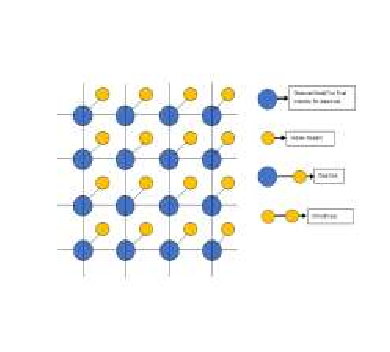
\includegraphics{mrf3.eps}
\caption{MRF Formulation for 4X4 node}
\label{fig:editpublish}
%\centerline{\epsffile{E:/Inderscience/LATEX-FILES/IJMSO/F4.eps}}
\end{figure}









\begin{equation}\label{}
    E (f)  =\sum_{i\in I}U_{i}(f_{i}) + \sum_{i,j\in N}V_{i,j}(f_{i},f_{j})
\end{equation}
Where
\begin{itemize}
 \item{E is Energy function}
  \item  {U is data cost function}








  \item {V is smoothness cost function }
  \item{i is pixel index }
  \item{j is neighboring index}
























\end{itemize}
The energy function adds all the cost at each link given in observed node Y with some disparity for each corresponding pixel in the hidden node X. The aim is to find the disparity from the hidden node, which produces lowest energy. \\To find lowest energy in the Markov network is NP hard and it means to get a solution for such problem takes unthinkably long time, which is because each pixel (node) in the disparity Map can take any value in the disparity space (state).The loopy Belief Propagation (LBP) algorithm is one of the many algorithms that can find an approximate solution for a MRF
























\subsection{Belief Propagation:}
The Belief Propagation algorithm was proposed by  \cite{pearl}.\\ Belief Propagation can be applied to graph which contains loops .The Loopy Belief Propagation is an approximate inference algorithm, which keeps passing messages around Markov state or node until a stable belief state is reached, so the Loopy Belief Propagation algorithm is an iterative algorithm and messages will converge on doing iterations.
























\subsubsection{In terms of Probabilistic theory}
The main steps in Belief propagation are as follows:
















\begin{itemize}
\item {After t iterations  $M^{(t)}_{i\rightarrow j}$ and $M ^{(t)}_{j\rightarrow i}$ are messages }
  \item {Messages take values in the space of probability distributions over a single variable space $\chi $}








  \item {$M^{(t)}_{i\rightarrow j}$ = \{ $M^{(t)}_{i\rightarrow j}$ $(x_{i}$): $x_{i}$ $\in$$\chi$\},with $M^{(t)}_{i\rightarrow j}$ $(x_{i}$)>0 ,$ \sum$ $M^{(t)}_{i\rightarrow j}$ $(x_{i}$)=1: }
\end{itemize}








The characteristic feature of Belief Propagation or message passing algorithm is that for a given node,  updates outgoing messages are on the basis of incoming ones at previous iteration   refer to \cite{Mezard}\\
The messages are updated in three different ways in Belief Propagation, which are known as Sum Product BP, Max Product BP and Minimum Sum BP.



\subsection{Message updates in Minimum sum Belief Propagation;}




To update message in minimum sum method is explained with help of Figure:2.

\begin{figure}[t]%4
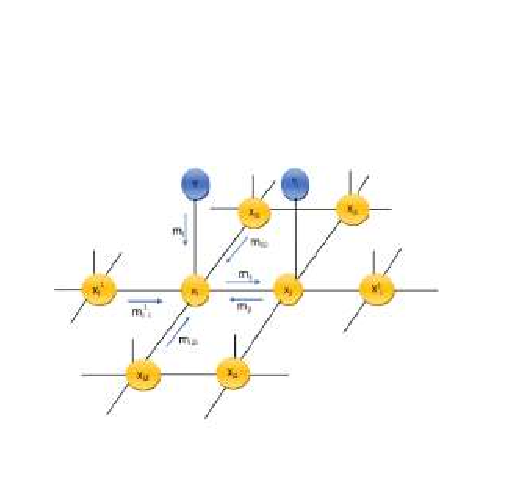
\includegraphics{bp.eps}
\caption{Description of Belief Propagation}\label{fig:editpublish}
%\label{fig:editpublish}
%centerline{\epsffile{E:/Inderscience/LATEX-FILES/IJMSO/F4.eps}}
\end{figure}
Yellow nodes with respect to above diagram are hidden nodes. Belief Propagation is applied to hidden nodes only.  Blue nodes are observed node.






The steps to find message passing  and belief for                 minimum sum method explained below:

$m_{i,j}$is  message passing from node i to node j: \\The message sent from node $ x_{i}$  to $x_{j}$ is given below:








\begin{equation}\label{}
m_{i,j}\leftarrow Min_{xi} + V_{i,j}(x_{i},x_{j})+  m^{1}_{i_i} +  m_{i}+ m_{i2i} +  m_{i1i} \\
\end{equation}








%m_{i,j}$ $\leftarrow $ $Min_{xi}$ + $V_{i,j}$$(x_{i}$,$x_{j}$)+  $m^{1}_{i_i}$ + $ m_{i}$ +$ m_{i2i}$ + $ m_{i1i}$ \\
The belief at $x_{i}$ is computed as:
\begin{equation}\label{}
b_{1}\leftarrow m^{1}_{i_i} +  m_{i}+ m_{i2i} + m_{i1i} + m_{j,i}
\end{equation}








































\subsection{The method used for simulation results}








The method used for our experiment in this paper is Minimum Sum Belief propagation .  The Minimum Sum BP algorithm finds the max marginal at each node the in log space. Minimum sum messages are defined to the overall additive constant.\\  Message initialization, message updates rule and finding beliefs are the main steps in Belief Propagation algorithm.\\
Messages in Minimum Sum BP algorithm are initialized to zero. The normalization of   message is not required for Minimum Sum BP because it operates in log space.\\
The message update rule








\begin{equation}\label{}
Msg_{i\rightarrow j}(d) = Min_{l'}\{(U_{y_{i},d})+ (V _{d,d'}) +\sum_{k\in i\setminus j} Msg_{k\rightarrow i}(d')\}
\end{equation}
\begin{itemize}
\item{$y_{i}$ is intensity value at pixel index.}\item{$ Msg_{i\rightarrow j}(d)$   messages from node i to j for disparity d } \item{ d is disparity range or level} \item { d' is disparity values belong to all disparity range or level } \item{   The disparity range or level is a variable of the form d = $2^{x}$ } \item{  U is data cost function, V is smoothness cost function }
\end{itemize}
The best assignment of disparity can be obtained by finding the belief which gives smallest value.
\begin{equation}\label{}
  belief({x}_{i}=d)) = \{(U_{y_{i},d}) + \sum_{k\in x_{i}} Msg_{k\rightarrow i}(d)
\end{equation}
\subsection{The models used }
The data cost function is sum of absolute difference function used.
\begin{equation}\label{}
    Data cost function (U) = \sum_{x,y} \{ | I_{x,y}- J_{x-d,y} |\}
\end{equation}
where
\begin{itemize}
\item{ I x ,y  is left image }
\item{ J x ,y  is right image } \item{ d is disparity range or level  }
\end{itemize}
The four connected grid is used for smoothness cost function.\\\     The four connected grid is used for smoothness cost function.
The equation for  Smoothness cost function (V) is given below:
\begin{equation}\label{}
f(v) = w \times min(|f |, t)
\end{equation}
Where w is tunable variable: t is truncation value:
%\begin{figure}[t]%4
%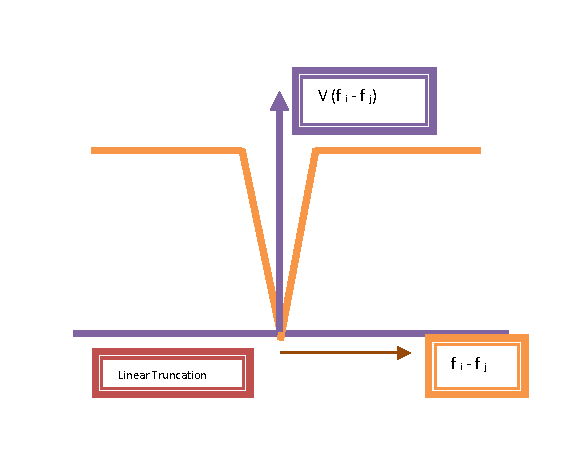
\includegraphics{linear2..eps}
%\caption{Linear Quadratic Model}
%\label{fig:editpublish}
%%centerline{\epsffile{E:/Inderscience/LATEX-FILES/IJMSO/F4.eps}}
%\end{figure}
\section{Experimental Results }
The test stereo input images Alovera, Baby, Pot and Tsukuba are from vision .middlebury.edu .The test stereo images are rectified and the radial distortion is removed. The ground truth image for each test stereo image is used for comparing performance of disparity map.The  system used for testing is Intel(R) Core(TM) i5-4200M CPU @2.5GH. And software used for programming is MATLAB version 15.\\
In the first method of evaluation process, the linear model is used as a smoothness cost function for Minimum Sum BP. The tunable variable parameter (w) is at 20 and truncation parameter (t) is at 2 which restricts the maximum value or as a threshold value.The  different  disparity range(x) used are16, 32, 64  and  number of iteration used in our method is10.\\ The disparity map for different disparity range for all test stereo images are shown figure:3.
The computational estimations  PSNR (Peak Signal to Noise Ratio),  in dB and MSE (Mean Square Error) per total number of pixel are shown in figure:4    and in figure:5 for all test stereo images as bar graph. The run time in seconds for all test stereo images is shown as a bar graph in figure:6.
\begin{figure}

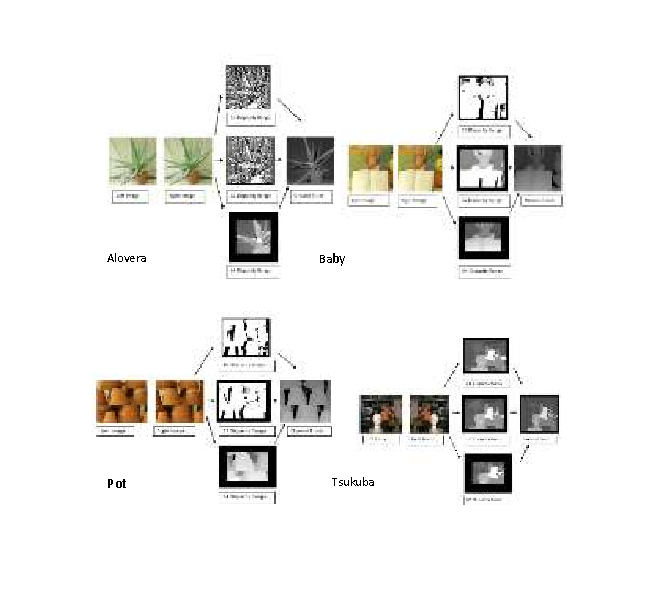
\includegraphics{figure4.eps}
\caption{ Disparity map for all test stereo images for different disparity Range}\label{fig:editpublish}
\end{figure}
\begin{figure}
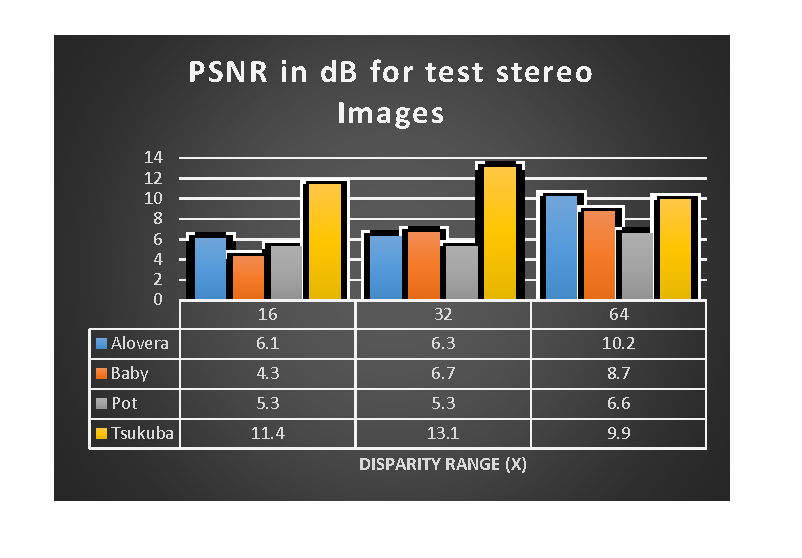
\includegraphics{psnrm.eps}
\caption{Graphical Representational for PSNR  for different Disparity range}\label{fig:editpublish}
\end{figure}
 \begin{figure}
  % Requires \usepackage{graphicx}
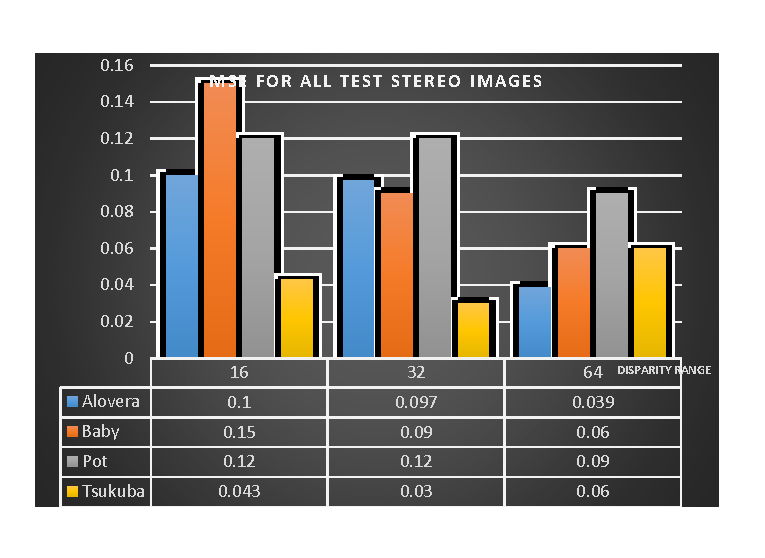
\includegraphics{msem.eps}
\caption{Graphical Representation for MSE  for different disparity Range}
\end{figure}
 \begin{figure}
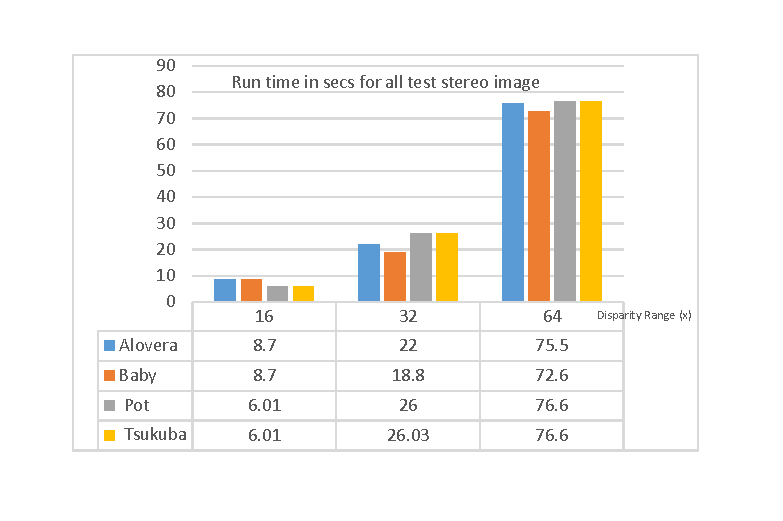
\includegraphics{runtime.eps}
\caption{Graphical Representation for Runtime different disparity Range}\label{fig:editpublish}
\end{figure} \\In second experimental process, The truncation parameter (t) is kept at constant one .The disparity range for Alovera , Baby and Pot kept at 64 whereas for Tsukuba it is at 32 for 10 iterations.\\The second method   is  tested for various values of tunable parameter(w) such as 0.1,0.2,1,5,10. The disparity map for different values of tunable parameter for all test stereo images are shown in figure:7 The bar graph representation  showing    computational estimations  PSNR (Peak Signal to Noise Ratio),  in dB and MSE (Mean Square Error) per total number of pixel are  in figure:8   and in figure:9 for all test stereo images for different values of  tunable parameter(w)
\begin{figure}
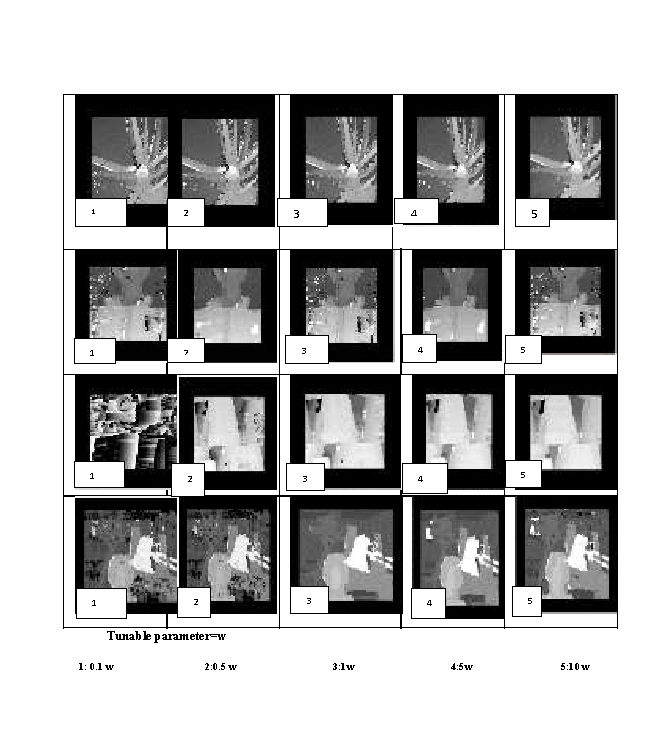
\includegraphics{differentw.eps}
\caption{Disparity map for different tunable variable}\label{fig:editpublish}
\end{figure}
\begin{figure}
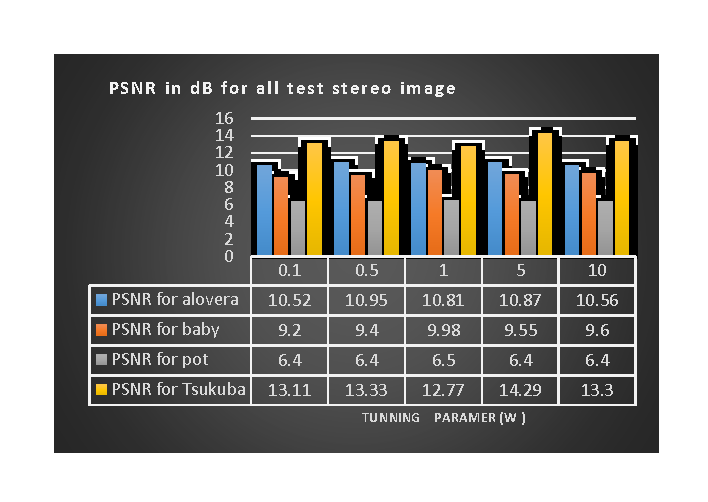
\includegraphics{psnrw.eps}
\caption{Graphical Representational for PSNR for different tunable variable}\label{fig:editpublish}
\end{figure}
\begin{figure}
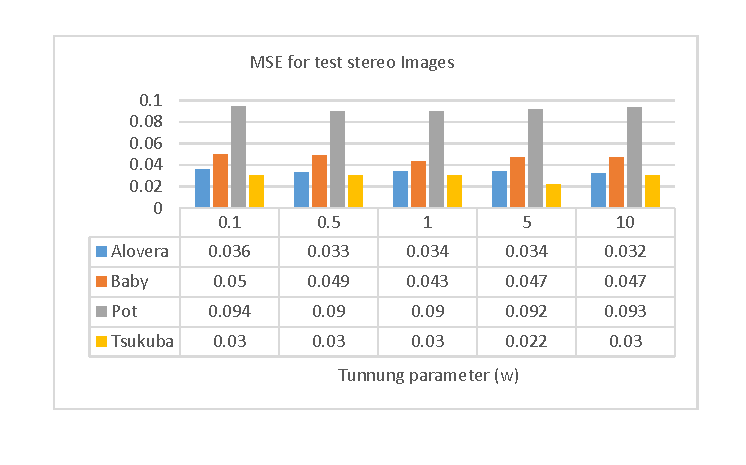
\includegraphics{msew.eps}
\caption{Graphical Representational for MSE for different tunable variable}\label{fig:editpublish}
\end{figure}
\section{Discussion}  %The first method of our experimental   analysis is for different disparity range for all test stereo images. The PSNR (Peak signal to noise ratio) for alovera is 6.1 dB, 6.3 dB, 10.2dB at disparity range 16, 32, 64 respectively. The MSE (mean square error) for the same is 0.1, 0.097, and 0.039 at disparity range 16, 32, 64 respectively. The computational analysis shows that for alovera maximum PSNR and Minimum MSE is obtained at disparity range 64. The optimal disparity map with respect to ground truth for alovara by our method is obtained at disparity range 64.\\
%In similar way for baby test stereo image PSNR is 4.3dB, 6.7dB and 8.7dB at disparity range 16, 32, 64 respectively. The MSE is 0.15, 0.09 and 0.06 at disparity range 16, 32, 64 respectively. The computational analysis for baby shows that maximum PSNR and Minimum MSE is obtained at disparity range 64.The  optimal disparity map with respect to ground truth for baby by our method  is  obtained at  64 disparity range .\\
%Similarly for Pot test stereo image PSNR is 5.3dB, 5.3dB and 6.6dB at disparity range 16, 32, 64 respectively. The MSE is 0.12, 0.12 and 0.09 at disparity range 16, 32, 64 respectively. The computational analysis for pot shows that maximum PSNR and Minimum MSE is obtained at disparity range 64.The optimal  disparity map for pot  also  obtained at  64 disparity range.\\
%Likewise for Tsukuba test stereo image PSNR is 11.4dB, 13.1 dB and 9.9dB at disparity range 16, 32, 64 respectively. The MSE is 0.043, 0.03 and 0.06 at disparity range 16, 32, 64 respectively. The computational analysis for Tsukuba shows that maximum PSNR and Minimum MSE is obtained at disparity Range 32 but as disparity range increases to 64 level PSNR decreases and MSE increases ,It shows that for Tsukuba optimal  disparity map with respect to ground truth  is obtained  at disparity range 32.\\
%To find run time of the algorithm by our method system used is  at a speed 2.5GHz. It shows that while increasing  disparity range  run time of the algorithm also increases. The run time by our method to get optimal disparity map for Alovera, Baby and  Pot  is at 76sec, 73sec,and 77sec  respectively, while for Tsukuba run time is 26sec because  optimum disparity map is  at disparity rang 32\\
%In the second method of experimental analysis the tunable parameter (w) from Quadratic linear model used as variable. The truncation (t) parameter is kept at constant one. After finding optimal disparity range from first method for all test stereo image. The disparity range is kept at 64 for alovera, baby and pot, for Tsukuba disparity range is kept at 32. The disparity map is computed for keeping tunable parameter at 0.1, 0.5,1,5,10.\\
%As tunable parameter (w) is increased from 0.1 to 10,computational estimates shows that for Alovera optimal disparity map obtained at 10 with PSNR 10.56dB and MSE is at 0.032.The optimal disparity map for baby is computed at tunable parameter (w)  5 with PSNR 9.55dB and MSE 0.043.\\
%The disparity map generated for pot at tunable parameter (w) is at 0.1 is very much distorted but as this parameter increased to higher value distortion in disparity map is reduced. The optimum disparity map for pot is obtained at tunable parameter (w) 1 with PSNR 6.5dB and MSE is at 0.09.\\
%The computational estimation for Tsukuba finds optimal disparity map at tunable parameter (w) 5 with PSNR 14.3dB and MSE is at 0.022.
%
%
%


The first method of our experimental   analysis is for different disparity range for all test stereo images.\\
The PSNR (Peak signal to noise ratio) for alovera is 6.1 dB at disparity range 16 with MSE (mean square error) 0.1 and run time 9 sec. While for same test stereo image disparity range is increased to 32, PSNR is 6.3 dB with MSE 0.097 and run time 22sec .On increasing disparity range to 64 PSNR for alovera is 10.2dB and MSE is 0.039 and run time 76sec.The optimal disparity map is achieved with respect to ground truth by our method using minimum sum belief propagation for alovera is   at disparity range 64 with high PSNR and low MSE for 10 iterations even though run time increases with disparity range.\\
In similar way for baby test stereo image at disparity range 16 PSNR is 4.3dB, MSE is 0.15 and run time is9sec. While for same test stereo image disparity range is increased to 32, PSNR is 6.7 dB with MSE 0.09 and run time 19 sec .On increasing disparity range to 64 PSNR for baby is 8.7dB and MSE is 0.06 and run time 77 sec. The optimal disparity map is achieved with respect to ground truth by our method using  minimum sum belief propagation  for baby  is   at disparity range 64 with high PSNR  and low MSE  for 10 iterations even though run time  increases with disparity range.\\
Similarly for Pot test stereo image at disparity range 16, PSNR is 5.3dB, MSE is 0.12 and runtime is 6 sec. As disparity range is increased to 32 for baby PSNR is 5.3dB, MSE is 0.12 and run time is 26sec.On increasing disparity range to 64 PSNR is 6.6dB, MSE is 0.09 and runtime is 73 sec. The optimal disparity map for pot also obtained at 64 disparity range with High PSNR and low MSE by our method for 10 iterations.\\
Likewise for Tsukuba test stereo image at disparity range 16 PSNR is 11.4dB, MSE is 0.043 and runtime is 6 sec. On increasing disparity range to 32 for Tsukuba PSNR is 13.1dB, MSE is 0.03 and run time is 26 sec. As disparity range is increased to 64, PSNR is decreased to 9.9dB, MSE is increased to 0.06 and run time is 77 sec. The optimal disparity map for Tsukuba is obtained by our method using minimum sum Belief Propagation with high PSNR and low MSE at disparity range 32 for 10 iterations.\\
In the second method of experimental analysis the tunable parameter (w) from Quadratic linear model used as variable. The truncation (t) parameter is kept at constant one. After finding optimal disparity range from first method for all test stereo image. The disparity range is kept at 64 for alovera, baby and pot, for Tsukuba disparity range is kept at 32. The disparity map is computed for keeping tunable parameter at 0.1, 0.5,1,5,10.\\
As tunable parameter (w) is increased from 0.1 to 10,computational estimates shows that for Alovera optimal disparity map is   obtained at tunable parameter (w) 10 with PSNR 10.56dB and  low MSE is at 0.032 for 10 iterations. The optimal disparity map for baby is computed at tunable parameter (w)  5 with PSNR 9.55dB and MSE  low at       0.043 for 10 iterations\\
The disparity map generated for pot at tunable parameter (w) is at 0.1 is very much distorted but as this parameter increased to higher value distortion in disparity map is reduced. The optimum disparity map for pot is obtained at tunable parameter (w) 1 with PSNR 6.5dB and MSE is at  low  0.09. for 10 iterations\\
The computational estimation for Tsukuba finds optimal disparity map at tunable parameter (w) 5 with PSNR 14.3dB and low  MSE is at 0.022    for 10 iterations








\section{Conclusion}
The method presented in this paper using minimum sum belief propagation computes disparity map in which objects are identified efficiently. In our method, belief propagation algorithm converge for Alovera ,baby and pot at disparity range 64 with less mean square error 0.039,0.06 and 0.09 respectively as well as  for Tsukuba it  converge at disparity range 32 with less mean square error 0.03.\\
Our results in second method of analysis shows that as per computational estimations and subjective analysis in accordance with  human perceptions for alovera, baby, pot and Tsukuba  disparity  map obtained  are as  commensurable to ground truth at tunable parameter (w) 10,5,1,5.The sharpness of the disparity map depends up on the value of parameter used in quadratic linear model.\\
The further study can be done on optimizing message updates method in belief propagation. Since sharpness of disparity map depends upon value of tunable parameter, fixing this value is challenging one further study can be done on these value.
















%%%%%%%%%%%%%%%%%%%%%%%%%%%%%%%%%%%%%%%%%%%%%%%%%%%%%%%%%%%%%%%%%%%%%%%%%%%%%%%%%%%%%








%\bibliography{ijmso}
%\bibliographystyle{unsrt}
%\bibliographystyle{alpha}
\begin{thebibliography}{10}
\bibitem[\protect\citeauthoryear{kuk-Jin Yoon and In Sokweon}{2010}]{KUKJINSOK}
L.kuk-Jin Yoon, In Sokweon   'Adaptive support -weight approach for correspondence search', {\it IEEE Trans- actions on pattern analysis and machine Intelligence},Vol. 28,no.4 pp 650-651
\bibitem[\protect\citeauthoryear{Patrik Kamencay,Martina}{2012}]{patrikkam}
Patrik Kamencay, Martina Zachariasova,Martin Brezman, Roman Jarina, Robert Hudec,Miroslav Benco, Slavomir Matuska(2012) 'A New Approach for Disparity Map Estimation from stereo Image Sequences using Hybrid Segmentation Algorithm', {\it International Journal of Modern Engineering Research},Vol.2,Issue 5,pp3201-3206


\bibitem[\protect\citeauthoryear{Yedidia                       }{1998}]{Yedidia         }
J.  S.  Yedidia,  W.  T.  Freeman,  and  Y.  Weiss                                                                                                                 (1998)                 Generalized  belief  propagation                                                                                        ', {\it 16.	Proc. NIPS                                            },pp. 689-695


\bibitem[\protect\citeauthoryear{Tappen and Freeman}{2003}]{TAPPEN}
Tappen,M.F. and Freeman,W.T(2003) 'Comparison of graph cuts with BP for stereo, using identical MRF parameters ', {\it IEEE International conference on computer vision.},



\bibitem[\protect\citeauthoryear{Pedro  F.  Felzenszwalb,Daniel  P.Huttenlocher}{2006}]{Pedro}
 Pedro  F.  Felzenszwalb,Daniel  P.Huttenlocher (2006) ' A  Efficient  Belief  Propagation  For Early Vision ', {\it    International Journal Of Computer Science}                                                           ,Vol. 41-54, No.2


\bibitem[\protect\citeauthoryear{ Yu-Chang Andnelson Chang  }{2006}]{chan}
 	Y. C. Tseng, N. Chang and T. S. Chang                                               (2007) ' Low Memory Cost Block-based Belief Propagation for Stereo Correspondence                           ', {\it  IEEE International Conference on Multimedia and Expo                                                                                                        },  pp. 1415-1418l.

\bibitem[\protect\citeauthoryear{Lian and Cheng                  }{2009}]{Liang}
	C. K. Liang, C. C. Cheng, Y. C. Lai, L. G. Chen and H. H. Chen                                                                                                                 (2009) 'Hardware Efficient Belief Propagation                                                                                                           ', {\it  Proc. of IEEE Conf. Computer Vision and Pattern Recognition                                                   },  pp. 80-87


\bibitem[\protect\citeauthoryear{nhiaho}{http://nghiaho.com}]{nhiaho}
http://nghiaho.com/notes/Markov Random Field, Loopy Belief Propagation, stereovision


\bibitem[\protect\citeauthoryear{Judea Pearl}{1998}]{pearl}
Judea Pearl(1998) `Probabilistic Reasoning in Intelligent Systems
', {\it Kaufmann Morgann Publishers, Second Revised And updated Edition      }.

\bibitem[\protect\citeauthoryear{Mezard M,Montanari} {2009}]{Mezard} Mezard (2009)`A Information , Physics and Computation', {\it A Information , Physics and Computation page 294}.


\bibitem[\protect\citeauthoryear{  Sun  Zheng           }{2003}]{sun}
	J.  Sun,  N.  N.  Zheng  and  H.  Y.  Shum                                                                                                                 (2003) ' Stereo  Matching  Using  Belief  Propagation                                                                                                          ', {\it  IEEE  Trans.  Pattern  Analysis  and  Machine  Intelligence                                                   },Vol.7,  no.  252,pp.787-800
\bibitem[\protect\citeauthoryear{SzeliskiPatrik Zabih                }{2008}]{Szeliski         }
	R. Szeliski, R. Zabih, D. Scharstein, O. Veksler, V. Kolmogorov, A. Agarwala, M. F. Tappen and C. Rother,                                                                              (2108)'A Comparative Study of Energy Minimization Methods for Markov Random Fields', {\it   IEEE Trans. Pattern Anal. Mach. Intell },Vol.6, no. 302,pp1068-1080

\bibitem[\protect\citeauthoryear{Freeman,E.C.,Pasztor                       }{}]{freeman  }
	W Freeman,E.C.,Pasztor and O.T.Carmichal                                                                                                                  'Learning Low level Vision                                                                                                            ', {\it In In- ternational journel of computer vision                                                    },40(1);25-47,2000

\bibitem[\protect\citeauthoryear{Li Zhou, Tao Sun                      }{2014}]{ Zhou,         }
	Li Zhou, Tao Sun, Yuanzhi Zhan and Jia Wang                                                                                                                 (2014) 'Software and Hardware Implemen- tations  of  Stereo  Matching                                                                                                           ', {\it IInternational  Journal  of  Electronics  and  Informatics                                                   },Vol.7, No.4 (2014), pp.37-562, No.1,

\bibitem[\protect\citeauthoryear{Anders                       }{2010}]{Anders         }
Anders  Olofsson                                                                                                                 (2010) 'Modern  Stereo  Correspondence  Algorithms: Investigation  and  eva- luation                                                                                                           ', {\it  Department  of  Electrocal  Engineering, Linkoping  University,s-581  83  Linkoping,Sweden }

\bibitem[\protect\citeauthoryear{Jianguo Ding                       }{2010}]{Jianguo Ding         }
Jianguo Ding                                                                                                                 (2010) 'Probabilistic Inferences In Bayesian Networks                         ', {\it International Journal Of Computer Science                                                    },Arxiv:1011.0935V2
\bibitem[\protect\citeauthoryear{github    }{http://github.com             }]{github    }
https://github.com/daviddoria/Tutorials/blob/master/BeliefPropagation/- BeliefPropagation.pdf
\bibitem[\protect\citeauthoryear{cedar    }{www.cedar.buffalo.edu                    }]{mirc}
http://www.cedar.buffalo.edu/srihari/CSE574/Chap8/Ch8- GraphicalModelInference/Ch8.3.3-Max-SumAlg.pdf              \bibitem[\protect\citeauthoryear{Erik      }{}]{Erik }	Erik. B. Sudderth and William T. Freeman                                                                                                                 () 'Signal And Image Processing With Belief Propagation                                                                                                           ', {\it Accepted To Appear In IEEE Signal Processing Magazine                                                    }, \bibitem[\protect\citeauthoryear{Frank R. Kschischang       }{2012}]{Frank R. Kschischang         }
	Frank R. Kschischang, Brendan J. Frey, Hans Andrea Loeliger                                                                                                                 (2001) 'A Factor Graph and The Sum Product Algorithm                                                                                                         ', {\it IEEE Transcations On Information Theory                                                    },Vol 47. No.2

\bibitem[\protect\citeauthoryear{Brad Hiebert-Treuer, Sarri Al Nashashibi, and Daniel Scharstein                                         }{
http://www.vision. Middlebury.edu  /}]{birn}
Brad Hiebert-Treuer, Sarri Al Nashashibi, and Daniel Scharstein  , http://www.vision. Middlebury.edu/


\end{thebibliography}
\end{document} 